%--------------------
% Packages
% -------------------
\documentclass[11pt,english]{article}
\usepackage{amsfonts}
\usepackage[left=2.5cm,top=2cm,right=2.5cm,bottom=3cm,bindingoffset=0cm]{geometry}
\usepackage{amsmath, amsthm, amssymb}
\usepackage{tikz}
\usetikzlibrary{calc}
\usetikzlibrary{decorations.pathreplacing,calligraphy}
\usepackage{fancyhdr}
%\usepackage{currfile}
\usepackage{nicefrac}
\usepackage{cite}
\usepackage{graphicx}
\usepackage{caption}
\usepackage{longtable}
\usepackage{rotating}
\usepackage{lscape}
\usepackage{booktabs}
\usepackage{float}
\usepackage{placeins}
\usepackage{setspace}
\usepackage[font=itshape]{quoting}
\onehalfspacing
\usepackage{mathrsfs}
\usepackage{tcolorbox}
\usepackage{xcolor}
\usepackage{subcaption}
\usepackage{float}
\usepackage[multiple]{footmisc}
\usepackage[T1]{fontenc}
\usepackage[sc]{mathpazo}
\usepackage{listings}
\usepackage{longtable}
\definecolor{cmured}{RGB}{175,30,45}
\definecolor{macroblue}{RGB}{56,108,176}
\usepackage[format=plain,
            labelfont=bf,
            textfont=]{caption}
\usepackage[colorlinks=true,citecolor=macroblue,linkcolor=macroblue,urlcolor=macroblue]{hyperref}
\usepackage{varioref}
\usepackage{chngcntr}
\usepackage{datetime}

\definecolor{darkgreen}{RGB}{30,175,88}
\definecolor{darkblue}{RGB}{30,118,175}
\definecolor{maroon}{rgb}{0.66,0,0}
\definecolor{darkgreen}{rgb}{0,0.69,0}

%Counters
\newtheorem{theorem}{Theorem}[section] 
\newtheorem{proposition}{Proposition}
\newtheorem{lemma}{Lemma}
\newtheorem{corollary}{Corollary}
\newtheorem{assumption}{Assumption}
\newtheorem{axiom}{Axiom}
\newtheorem{case}{Case}
\newtheorem{claim}{Claim}
\newtheorem{condition}{Condition}
\newtheorem{definition}{Definition}
\newtheorem{example}{Example}
\newtheorem{notation}{Notation}
\newtheorem{remark}{Remark}


\hypersetup{ 	
pdfsubject = {},
pdftitle = {TidyTuesday Week 43},
pdfauthor = {Pranay Gundam},
linkcolor= macroblue
}


\title{\textbf{TidyTuesday Week 43}}
\author{Pranay Gundam}


%-----------------------
% Begin document
%-----------------------
\begin{document}

\maketitle

\tableofcontents

\section{Weekly Summary}


\section{Date: 2024-10-21}
\noindent \textbf{Series ID: CGDPESMZA666NRUG} 

\noindent This series is titled Expenditure-side Real GDP at Current Purchasing Power Parities for Mozambique and has a frequency of Annual. The units are Millions of 2017 U.S. Dollars and the seasonal adjustment is Not Seasonally Adjusted.The observation start date is 1960-01-01 and the observation end date is 2019-01-01.The popularity of this series is 1. \\ 

\noindent \textbf{Series ID: IR14200} 

\noindent This series is titled Import Price Index (End Use): Bauxite and Aluminum and has a frequency of Monthly. The units are Index 2000=100 and the seasonal adjustment is Not Seasonally Adjusted.The observation start date is 1986-09-01 and the observation end date is 2024-09-01.The popularity of this series is 38. \\ 

\subsection{Regression Tables and Plots}
\begin{center}
\begin{tabular}{lclc}
\toprule
\textbf{Dep. Variable:}                & value\_fred\_IR14200 & \textbf{  R-squared:         } &     0.588   \\
\textbf{Model:}                        &         OLS          & \textbf{  Adj. R-squared:    } &     0.571   \\
\textbf{Method:}                       &    Least Squares     & \textbf{  F-statistic:       } &     34.30   \\
\textbf{Date:}                         &   Mon, 21 Oct 2024   & \textbf{  Prob (F-statistic):} &  4.85e-06   \\
\textbf{Time:}                         &       13:41:09       & \textbf{  Log-Likelihood:    } &   -109.92   \\
\textbf{No. Observations:}             &            26        & \textbf{  AIC:               } &     223.8   \\
\textbf{Df Residuals:}                 &            24        & \textbf{  BIC:               } &     226.3   \\
\textbf{Df Model:}                     &             1        & \textbf{                     } &             \\
\textbf{Covariance Type:}              &      nonrobust       & \textbf{                     } &             \\
\bottomrule
\end{tabular}
\begin{tabular}{lcccccc}
                                       & \textbf{coef} & \textbf{std err} & \textbf{t} & \textbf{P$> |$t$|$} & \textbf{[0.025} & \textbf{0.975]}  \\
\midrule
\textbf{const}                         &      66.0597  &        9.716     &     6.799  &         0.000        &       46.006    &       86.113     \\
\textbf{value\_fred\_CGDPESMZA666NRUG} &       0.0023  &        0.000     &     5.857  &         0.000        &        0.002    &        0.003     \\
\bottomrule
\end{tabular}
\begin{tabular}{lclc}
\textbf{Omnibus:}       &  0.668 & \textbf{  Durbin-Watson:     } &    1.165  \\
\textbf{Prob(Omnibus):} &  0.716 & \textbf{  Jarque-Bera (JB):  } &    0.640  \\
\textbf{Skew:}          &  0.334 & \textbf{  Prob(JB):          } &    0.726  \\
\textbf{Kurtosis:}      &  2.620 & \textbf{  Cond. No.          } & 7.00e+04  \\
\bottomrule
\end{tabular}
%\caption{OLS Regression Results}
\end{center}

Notes: \newline
 [1] Standard Errors assume that the covariance matrix of the errors is correctly specified. \newline
 [2] The condition number is large,  7e+04. This might indicate that there are \newline
 strong multicollinearity or other numerical problems.

\begin{figure}
\centering
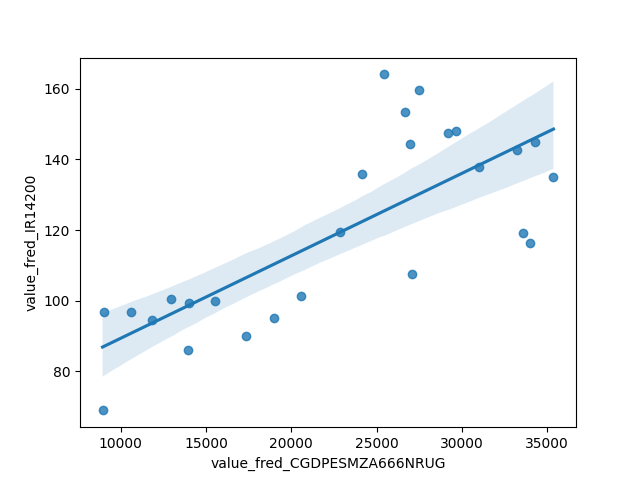
\includegraphics[scale = 0.9]{plots/plot_2024-10-21.png}
\caption{Regression Plot for 2024-10-21}
\end{figure}
\newpage

\include{tex_things/day_2024-10-22}
\section{Date: 2024-10-23}
\noindent \textbf{Series ID: RGDPTETRA629NUPN} 

\noindent This series is titled Purchasing Power Parity Converted GDP Laspeyres per person counted in total employment for Turkey and has a frequency of Annual. The units are 2005 International Dollars per Person Counted in Total Employment and the seasonal adjustment is Not Seasonally Adjusted.The observation start date is 1950-01-01 and the observation end date is 2010-01-01.The popularity of this series is 1. \\ 

\noindent \textbf{Series ID: BUSAANITL} 

\noindent This series is titled Banks in U.S.-Affiliated Areas; Net Interbank Transactions; Liability, Level (DISCONTINUED)" and has a frequency of Quarterly. The units are Millions of Dollars and the seasonal adjustment is Not Seasonally Adjusted.The observation start date is 1945-10-01 and the observation end date is 2024-01-01.The popularity of this series is 1. \\ 

\subsection{Regression Tables and Plots}
\begin{center}
\begin{tabular}{lclc}
\toprule
\textbf{Dep. Variable:}                & value\_fred\_BUSAANITL & \textbf{  R-squared:         } &     0.304   \\
\textbf{Model:}                        &          OLS           & \textbf{  Adj. R-squared:    } &     0.291   \\
\textbf{Method:}                       &     Least Squares      & \textbf{  F-statistic:       } &     23.62   \\
\textbf{Date:}                         &    Wed, 23 Oct 2024    & \textbf{  Prob (F-statistic):} &  1.05e-05   \\
\textbf{Time:}                         &        13:08:03        & \textbf{  Log-Likelihood:    } &   -469.36   \\
\textbf{No. Observations:}             &             56         & \textbf{  AIC:               } &     942.7   \\
\textbf{Df Residuals:}                 &             54         & \textbf{  BIC:               } &     946.8   \\
\textbf{Df Model:}                     &              1         & \textbf{                     } &             \\
\textbf{Covariance Type:}              &       nonrobust        & \textbf{                     } &             \\
\bottomrule
\end{tabular}
\begin{tabular}{lcccccc}
                                       & \textbf{coef} & \textbf{std err} & \textbf{t} & \textbf{P$> |$t$|$} & \textbf{[0.025} & \textbf{0.975]}  \\
\midrule
\textbf{const}                         &     -92.5528  &      329.111     &    -0.281  &         0.780        &     -752.380    &      567.274     \\
\textbf{value\_fred\_RGDPTETRA629NUPN} &      -0.0821  &        0.017     &    -4.860  &         0.000        &       -0.116    &       -0.048     \\
\bottomrule
\end{tabular}
\begin{tabular}{lclc}
\textbf{Omnibus:}       & 17.518 & \textbf{  Durbin-Watson:     } &    0.127  \\
\textbf{Prob(Omnibus):} &  0.000 & \textbf{  Jarque-Bera (JB):  } &   21.004  \\
\textbf{Skew:}          & -1.431 & \textbf{  Prob(JB):          } & 2.75e-05  \\
\textbf{Kurtosis:}      &  3.899 & \textbf{  Cond. No.          } & 4.46e+04  \\
\bottomrule
\end{tabular}
%\caption{OLS Regression Results}
\end{center}

Notes: \newline
 [1] Standard Errors assume that the covariance matrix of the errors is correctly specified. \newline
 [2] The condition number is large, 4.46e+04. This might indicate that there are \newline
 strong multicollinearity or other numerical problems.

\begin{figure}
\centering
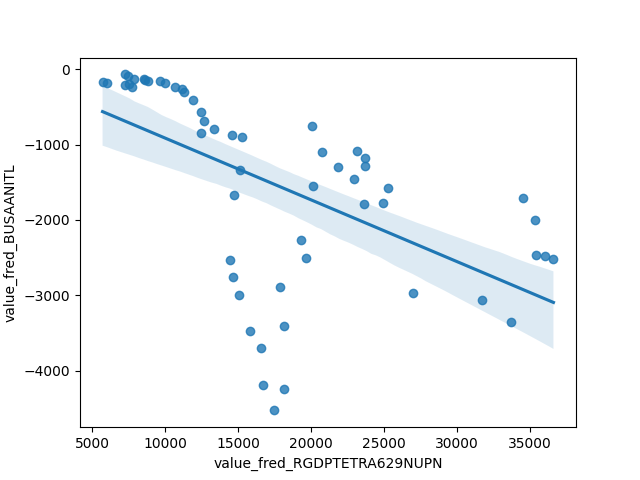
\includegraphics[scale = 0.9]{plots/plot_2024-10-23.png}
\caption{Regression Plot for 2024-10-23}
\end{figure}
\newpage

\section{Date: 2024-10-24}
\noindent \textbf{Series ID: NHSUSSP75OQP} 

\noindent This series is titled New Houses Sold by Sales Price in the United States, Between $750,000 and Over (DISCONTINUED) and has a frequency of Quarterly. The units are Percent and the seasonal adjustment is Not Seasonally Adjusted.The observation start date is 2002-01-01 and the observation end date is 2024-01-01.The popularity of this series is 1. \\ 

\noindent \textbf{Series ID: PCAGDPPLA646NWDB} 

\noindent This series is titled Gross Domestic Product Per Capita for Poland and has a frequency of Annual. The units are Current U.S. Dollars and the seasonal adjustment is Not Seasonally Adjusted.The observation start date is 1990-01-01 and the observation end date is 2023-01-01.The popularity of this series is 6. \\ 

\subsection{Regression Tables and Plots}
\begin{center}
\begin{tabular}{lclc}
\toprule
\textbf{Dep. Variable:}            & value\_fred\_PCAGDPPLA646NWDB & \textbf{  R-squared:         } &     0.600   \\
\textbf{Model:}                    &              OLS              & \textbf{  Adj. R-squared:    } &     0.580   \\
\textbf{Method:}                   &         Least Squares         & \textbf{  F-statistic:       } &     30.06   \\
\textbf{Date:}                     &        Thu, 24 Oct 2024       & \textbf{  Prob (F-statistic):} &  2.29e-05   \\
\textbf{Time:}                     &            11:47:05           & \textbf{  Log-Likelihood:    } &   -204.05   \\
\textbf{No. Observations:}         &                 22            & \textbf{  AIC:               } &     412.1   \\
\textbf{Df Residuals:}             &                 20            & \textbf{  BIC:               } &     414.3   \\
\textbf{Df Model:}                 &                  1            & \textbf{                     } &             \\
\textbf{Covariance Type:}          &           nonrobust           & \textbf{                     } &             \\
\bottomrule
\end{tabular}
\begin{tabular}{lcccccc}
                                   & \textbf{coef} & \textbf{std err} & \textbf{t} & \textbf{P$> |$t$|$} & \textbf{[0.025} & \textbf{0.975]}  \\
\midrule
\textbf{const}                     &    8026.9610  &     1055.160     &     7.607  &         0.000        &     5825.935    &     1.02e+04     \\
\textbf{value\_fred\_NHSUSSP75OQP} &    1224.5177  &      223.352     &     5.482  &         0.000        &      758.614    &     1690.421     \\
\bottomrule
\end{tabular}
\begin{tabular}{lclc}
\textbf{Omnibus:}       &  3.483 & \textbf{  Durbin-Watson:     } &    0.653  \\
\textbf{Prob(Omnibus):} &  0.175 & \textbf{  Jarque-Bera (JB):  } &    1.565  \\
\textbf{Skew:}          & -0.281 & \textbf{  Prob(JB):          } &    0.457  \\
\textbf{Kurtosis:}      &  1.821 & \textbf{  Cond. No.          } &     8.91  \\
\bottomrule
\end{tabular}
%\caption{OLS Regression Results}
\end{center}

Notes: \newline
 [1] Standard Errors assume that the covariance matrix of the errors is correctly specified.

\begin{figure}
\centering
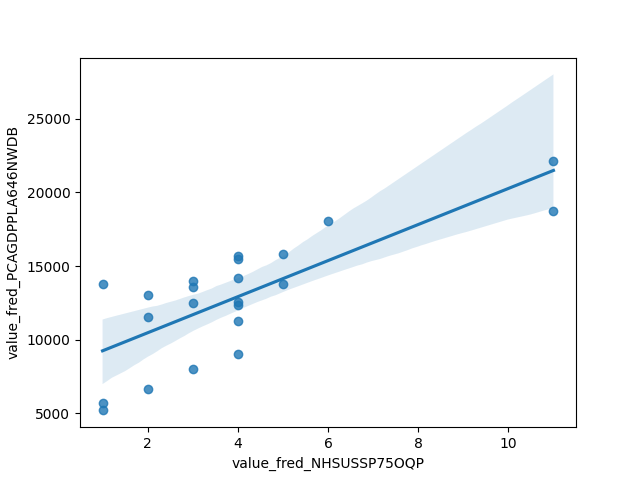
\includegraphics[scale = 0.9]{plots/plot_2024-10-24.png}
\caption{Regression Plot for 2024-10-24}
\end{figure}
\newpage

\include{tex_things/day_2024-10-25}
\include{tex_things/day_2024-10-26}
\section{Date: 2024-10-27}
\noindent \textbf{Series ID: MAABSNNB} 

\noindent This series is titled Nonfinancial Noncorporate Business; Total Miscellaneous Assets, Excluding Noncorporate Farms, Level (DISCONTINUED) and has a frequency of Quarterly, End of Period. The units are Billions of Dollars and the seasonal adjustment is Not Seasonally Adjusted.The observation start date is 1949-10-01 and the observation end date is 2015-01-01.The popularity of this series is 1. \\ 

\noindent \textbf{Series ID: DNSLAL} 

\noindent This series is titled Domestic Nonfinancial Sectors; Debt Securities; Liability, Level and has a frequency of Quarterly. The units are Millions of Dollars and the seasonal adjustment is Not Seasonally Adjusted.The observation start date is 1945-10-01 and the observation end date is 2024-04-01.The popularity of this series is 4. \\ 

\subsection{Regression Tables and Plots}
\begin{center}
\begin{tabular}{lclc}
\toprule
\textbf{Dep. Variable:}        & value\_fred\_DNSLAL & \textbf{  R-squared:         } &     0.899   \\
\textbf{Model:}                &         OLS         & \textbf{  Adj. R-squared:    } &     0.899   \\
\textbf{Method:}               &    Least Squares    & \textbf{  F-statistic:       } &     2261.   \\
\textbf{Date:}                 &   Sun, 27 Oct 2024  & \textbf{  Prob (F-statistic):} & 1.88e-128   \\
\textbf{Time:}                 &       11:23:12      & \textbf{  Log-Likelihood:    } &   -4040.8   \\
\textbf{No. Observations:}     &           256       & \textbf{  AIC:               } &     8086.   \\
\textbf{Df Residuals:}         &           254       & \textbf{  BIC:               } &     8093.   \\
\textbf{Df Model:}             &             1       & \textbf{                     } &             \\
\textbf{Covariance Type:}      &      nonrobust      & \textbf{                     } &             \\
\bottomrule
\end{tabular}
\begin{tabular}{lcccccc}
                               & \textbf{coef} & \textbf{std err} & \textbf{t} & \textbf{P$> |$t$|$} & \textbf{[0.025} & \textbf{0.975]}  \\
\midrule
\textbf{const}                 &    1.656e+06  &     1.25e+05     &    13.242  &         0.000        &     1.41e+06    &      1.9e+06     \\
\textbf{value\_fred\_MAABSNNB} &    6960.0780  &      146.385     &    47.546  &         0.000        &     6671.795    &     7248.361     \\
\bottomrule
\end{tabular}
\begin{tabular}{lclc}
\textbf{Omnibus:}       & 10.407 & \textbf{  Durbin-Watson:     } &    0.008  \\
\textbf{Prob(Omnibus):} &  0.005 & \textbf{  Jarque-Bera (JB):  } &    8.720  \\
\textbf{Skew:}          &  0.369 & \textbf{  Prob(JB):          } &   0.0128  \\
\textbf{Kurtosis:}      &  2.476 & \textbf{  Cond. No.          } &     982.  \\
\bottomrule
\end{tabular}
%\caption{OLS Regression Results}
\end{center}

Notes: \newline
 [1] Standard Errors assume that the covariance matrix of the errors is correctly specified.

\begin{figure}
\centering
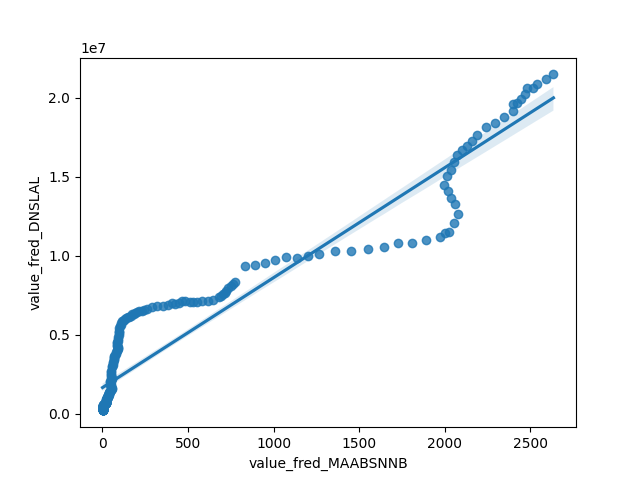
\includegraphics[scale = 0.9]{plots/plot_2024-10-27.png}
\caption{Regression Plot for 2024-10-27}
\end{figure}
\newpage


\end{document}
